
\section{Reproducing the ``stage 2" methods: CAM-based, feature-split, and strong baselines} \label{sec:stage2}

In this section, we describe our efforts in reproducing methods that aim to mitigate contextual bias: namely, the \emph{CAM-based} and \emph{feature-split} methods proposed by the original authors  (Figure~\ref{fig:overview}) and 7 other strong baselines. These are referred to as ``stage 2" methods because they are trained on top of the ``stage 1" \emph{standard} model (except for one strong baseline). Apart from the \emph{feature-split} method, which we discussed with the authors, all other implementations were based entirely on our interpretation of their descriptions in the original paper.

\begin{figure}[h!]
    \centering
    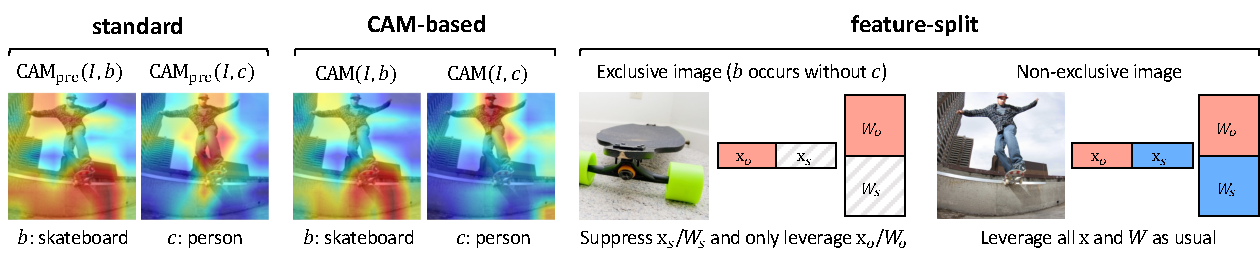
\includegraphics[width=1.0\linewidth]{../openreview/images/algorithms_final.pdf}
    \caption{Overview of the proposed methods. The \emph{CAM-based} methods enforces a minimal overlap between the ($b$, $c$) CAMs, while preventing them from drifting too far from CAM$_{\text{pre}}$ (CAMs of the \emph{standard} model). The \emph{feature-split} method suppresses context for exclusive images by disabling backpropagation through $W_s$ and setting $\mathrm{x}_s$ to a constant value; for non-exclusive images, it uses everything as usual.}
    \label{fig:overview}
\end{figure}


\subsection{The first proposed \textit{CAM-based} method} \label{sec:cam}

The \emph{CAM-based} method operates on the following premise: as $b$ almost always co-occurs with $c$, the network may learn to inadvertently rely on pixels corresponding to $c$ to predict $b$. The paper hypothesizes that one way to overcome this issue is to explicitly force the network to rely less on $c$'s pixel regions. This method uses class activation maps (CAMs)~\cite{zhou2015cnnlocalization} as a proxy for object localization information. For an image $I$ and category $r$, CAM($I$, $r$) indicates the discriminative image regions used by a deep network to identify $r$. For each biased category pair ($b$, $c$), a minimal overlap of their CAMs is enforced via the loss term:
\begin{equation} \label{eq:Lo}
    L_O = \textstyle\sum_{I \in \mathbb{I}_b 	\cap \mathbb{I}_c} \text{CAM}(I, b) \odot \text{CAM}(I, c),
\end{equation}
where $\odot$ denotes element-wise multiplication and $\mathbb{I}_b \cap \mathbb{I}_c$ is a set of images where both $b$ and $c$ appear. To prevent a trivial solution where the CAMs of $b$ and $c$ drift apart from the actual pixel regions, the paper uses a regularization term to keep the category's CAMs close to CAM$_{\text{pre}}$, produced using a separate network trained offline:
\begin{equation}
    L_R = \textstyle\sum_{I \in \mathbb{I}_b 	\cap \mathbb{I}_c} |\text{CAM}_\text{pre}(I, b) - \text{CAM}(I, b)| + |\text{CAM}_\text{pre}(I, c) - \text{CAM}(I, c)|.
\end{equation}
In our implementation, we separate a batch into two small batches during training, one with and one without co-occurrences. A sample is put into the \emph{co-occurrence} batch if any of the 20 biased categories co-occurs with its context. For the co-occurrence batch, we compute CAM with the current model being trained and CAM$_{\text{pre}}$ with the trained \emph{standard} model, using the official CAM implementation: \url{https://github.com/zhoubolei/CAM}. We update the model parameters with the following loss, where $L_\text{BCE}$ is the binary cross entropy loss:
\begin{equation}\label{eq:cam}
L_\text{CAM} = \lambda_1 L_O + \lambda_2 L_R + L_\text{BCE}.
\end{equation}
For the \emph{other} batch without any co-occurrences, we update the model parameters with $L_\text{BCE}$. 
With the hyperparameters reported in the paper, $\lambda_1$=0.1 and $\lambda_2$=0.01, we got underwhelming results and degenerate CAMs that drifted far from the actual pixel regions. Hence, we tried increasing the regularization weight $\lambda_2$ (0.01, 0.05, 0.1, 0.5, 1.0, 5.0) and achieved the best results with $\lambda_2$=0.1, which are reported in Table~\ref{tab:mainresults}. 

\subsection{The second proposed \emph{feature-split} method}

By discouraging mutual spatial overlap, the \emph{CAM-based} approach may not be able to leverage useful information from the pixel regions surrounding the context. Thus, the paper proposes a second method that splits the feature space into two subspaces to separately represent category and context, while posing no constraints on their spatial extents. Specifically, they propose using a dedicated feature subspace to learn examples of biased categories appearing without their context.\\
\\
Given a deep neural network, let $\mathrm{x}$ denote the $D$-dimensional output of the final pooling layer just before the fully-connected (fc) layer. Let the weight matrix associated with fc layer be $W \in R^{D \times M}$, where $M$ denotes the number of categories given a multi-label dataset. The predicted scores inferred by a classifier (ignoring the bias term) are $\hat{y}=W^T \mathrm{x}$. To separate the feature representations of a biased category from its context, the paper does a random row-wise split of $W$ into two disjoint subsets: $W_o$ and $W_s$ (dimension $\frac{D}{2}\times M$).\footnote{In an email, the authors noted that a random split is not critical; they obtained similar results with a random split and a middle split. We observed that a middle split of $W$ yields better results for COCO-Stuff and DeepFashion, but the opposite for AwA. As the gains from using a middle split for COCO-Stuff and DeepFashion were larger than the losses for AwA, we use a middle split throughout our experiments.} Consequently, $\mathrm{x}$ is split into $\mathrm{x}_o$ and $\mathrm{x}_s$, and $\hat{y}=W^T_o \mathrm{x}_o + W^T_s \mathrm{x}_s$. When a biased category occurs without its context, the paper disables backpropagation through $W_s$, forcing the network to learn only through $W_o$, and set $\mathrm{x}_s$ to $\bar{\mathrm{x}}_s$ (the average of $\mathrm{x}_s$ over the last 10 mini-batches).\\
\\
We implemented the \emph{feature-split} method based on additional discussions with the original authors, to ensure that we replicated their method as closely as possible. For a single training batch, we first forwarded the entire batch through the model to obtain one set of scores $\hat{y}_{\text{non-exclusive}}=W^T_o \mathrm{x}_o + W^T_s \mathrm{x}_s$ and the corresponding features from the avgpool layer, which directly precedes the fc layer. 
We made a separate copy of these features and replaced $\mathrm{x}_s$ with $\bar{\mathrm{x}}_s$, then calculated a new set of output scores $\hat{y}_{\text{exclusive}} = W^T_o \mathrm{x}_o + W^T_s \bar{\mathrm{x}}_s$. Separate loss tensors for each of these outputs were computed, and elements corresponding to the exclusive and non-exclusive examples in the unmodified and modified loss tensors were zeroed out, respectively. The final loss tensor was obtained by adding these two together, and standard backpropagation was done using this final loss tensor. The gradients were calculated with respect to a weighted binary cross entropy loss:
\begin{equation}
    L_\text{WBCE} = - \alpha \big[t\log(\sigma(\hat{y})) + (1-t)\log(1-\sigma(\hat{y}))\big],
\end{equation}
where $t$ is the ground-truth label, $\sigma$ is the sigmoid function, and $\alpha$ is the ratio between the number of training images in which a biased category occurs in the presence of its context and the number of images in which it occurs in the absence of its context. A higher value of $\alpha$ indicates more data skewness.\footnote{In practice, the paper ensures $\alpha$ is at least $\alpha_{\text{min}}$, which they set to 3 for COCO-Stuff and AwA and 5 for DeepFashion. However, we found that most of the paper's biased category pairs have $\alpha$ smaller than $\alpha_{\text{min}}$. Out of 20 pairs, 13 pairs for COCO-Stuff, 20 pairs for DeepFashion, and 19 pairs for AwA had $\alpha$ smaller than $\alpha_{\text{min}}$. We also tried using higher values of $\alpha_{\text{min}}$ but didn't gain meaningful improvements, so we report results with the original authors' $\alpha_{\text{min}}$.}


\subsection{Strong baselines}
\label{sec:strong-baselines}

In addition to the \emph{standard} model, the paper compares the proposed methods with several competitive \textit{strong baselines}.

%[leftmargin=*] \setlength\itemsep{0em}
\begin{enumerate} 
	\item \textbf{Remove co-occur labels}: For each $b$, remove the $c$ label for images in which $b$ and $c$ co-occur.
    \item \textbf{Remove co-occur images}: Remove training instances where any $b$ and $c$ co-occur. For COCO-Stuff, this process removes 29,332 images and leaves 53,451 images in the training set.
    \item \textbf{Split-biased}: Split each $b$ into two classes: 1) $b \setminus c$ and 2) $b \cap c$.  Unlike other ``stage 2" models, this model is trained from scratch rather than on top of the \textit{standard} baseline because it has 20 additional classes. We later confirmed with the authors that they did the same.
    \item \textbf{Weighted loss}: For each $b$, apply 10 times higher weight to the loss for class $b$ when $b$ occurs exclusively.
    \item \textbf{Negative penalty}: For each $(b, c)$, apply a large negative penalty to the loss for class $c$ when $b$ occurs exclusively. In our email communication, the authors said that the negative penalty means a 10 times higher weight to the loss.
    \item \textbf{Class-balancing loss}~\cite{Cui_2019_CVPR}: For each $b$, put the images in three groups: exclusive, co-occurring, and other. The weight for each group is $(1-\beta)/(1-\beta^n)$ where $n$ is the number of images for each group and $\beta$ is a hyperparameter. The authors said they set $\beta=0.99$ in our email communication.
    \item \textbf{Attribute decorrelation}~\cite{Jayaraman_2014_CVPR}: Use the proposed method, but replace the hand-crafted features used in ~\cite{Jayaraman_2014_CVPR} with deep network features (i.e., conv5 features of a trained ``stage 1" ResNet-50).
\end{enumerate}


\subsection{Training details and computational requirements}

We trained all ``stage 2" models on top of the \emph{standard} model for 20 epochs using a learning rate of 0.01, a batch size of 200, and SGD with 0.9 momentum. The exceptions are \emph{split-biased} which is not trained on top of the \emph{standard} model and is thus trained for an additional 20 epochs to ensure a fair comparison; and \emph{CAM-based} which uses a batch size of 100 due to memory limits. All models were trained on a single RTX 3090 GPU and evaluated on the last epoch. On COCO-Stuff, the single-epoch training time was around 12.9 minutes for \emph{standard}, \emph{remove labels}, \emph{split-biased}, \emph{weighted}, \emph{negative penalty}, and \emph{class-balancing}. It took 8.4 minutes to train \emph{remove images}, and 17.3 minutes and 13.3 minutes to train \emph{CAM-based} and \emph{feature-split}, respectively. Thus, we reach a different conclusion from the paper's claim that the ``overall training time of both proposed methods is very close to that of a standard classifier." We suspect that this difference is due to the difference in implementation. Overall, the total training time for each method range from 35-43 hours on COCO-Stuff, 22-29 hours on DeepFashion, and 7-8 hours on AwA. For inference, the paper reports that a single forward pass of an image takes 0.2ms on a single Titan X GPU for the \emph{standard}, \emph{CAM-based}, and \emph{feature-split} methods. We confirmed that it takes the same amount of time for the three methods. See Appendix~\ref{sec:computationalrequirements} for detailed training and inference times.


\begin{table}[t!]
\centering
\caption{Performance of different methods on COCO-Stuff, DeepFashion, AwA, and UnRel on ``exclusive" and ``co-occur" distributions with best results in bold. We compare our results to the paper's results, specifically its  Table 2, 3, 4, 5, 8, 9. Per-category results can be found in Appendix~\ref{sec:percategory}.}
\label{tab:mainresults}
\resizebox{\linewidth}{!}{
\begin{tabular}{|c|cc|cc|cc|cc|cc|cc|cc|}
\hline
\multirow{3}{*}{Method} & \multicolumn{4}{c|}{COCO-Stuff (mAP)} & \multicolumn{4}{c|}{DeepFashion (top-3 recall)} & \multicolumn{4}{c|}{AwA (mAP)} & \multicolumn{2}{c|}{UnRel (mAP)} \\
\cline{2-15}
& \multicolumn{2}{c|}{Exclusive} & \multicolumn{2}{c|}{Co-occur} & \multicolumn{2}{c|}{Exclusive} & \multicolumn{2}{c|}{Co-occur} & \multicolumn{2}{c|}{Exclusive} & \multicolumn{2}{c|}{Co-occur} & \multicolumn{2}{c|}{3 categories} \\
\cline{2-15}
& Paper & Ours & Paper & Ours & Paper & Ours & Paper & Ours & Paper & Ours & Paper & Ours & Paper & Ours \\
\hline
\textit{standard\tablefootnote{To ensure a fair comparison with the "stage 2" models, we tried training the \emph{standard} model for an additional 20 epochs but did not see improvements; hence, we report the \emph{standard} results from Table~\ref{tab:baseline}.}}          & 24.5 & 23.9 & \textbf{66.2} & \textbf{65.0} & 4.9 & 7.0 & 17.8 & 22.8 & 19.4 & 19.5 & 72.2 & 69.0 & 42.0 & 43.0 \\
\hline
\textit{remove labels}     & 25.2 & 24.5 & 65.9 & 64.6 & 6.0 &  7.5   & \textbf{20.4} & 24.4 & 19.1 & 18.9 & 62.9 & 63.2 & -    & 42.7 \\
\textit{remove images}     & 28.4 & \textbf{29.0} & 28.7 & 59.6 & 4.2 &  5.6  & 5.4  & 13.0  & \textbf{22.7} & \textbf{21.7} & 58.3 & 65.2 & -    & 48.6 \\
\textit{split-biased}      & 19.1 & 25.4 & 64.3 & 64.7 & 3.5 & 4.9  & 14.3 & 11.1 & 19.7 & 18.2 & 66.8 & 64.2 & -    & 29.2 \\
\textit{weighted}          & \textbf{30.4} & 28.5 & 60.8 & 60.0 & -   & \textbf{29.5}    & -    & \textbf{43.6} & -    & 20.0 & -    & 67.7 & -    & 44.4 \\
\textit{negative penalty}  & 23.8 & 23.9 & 66.1 & 64.7 & 5.5 &  7.8  & 18.9 & 23.8  & 19.2 & 19.6 & 68.4 & 69.0 & -    & 42.5 \\
\textit{class-balancing}   & 25.0 & 24.6 & 66.1 & 64.7 & 5.2 &  8.0   & 19.4 & 24.8  & 20.4 & 19.9 & 68.4 & 68.2 & -    & 42.3 \\
\textit{attribute decorr.} & -    & -    & -    & -    & -   & -   & -    & - & 18.4 & 20.6 & 70.2 & \textbf{69.8} & -    & - \\
\hline
\textit{CAM-based}         & 26.4 & 26.9 & 64.9 & 64.2 & -   & -   & -    & - & -    & -    & -    & -    & 45.3 & 46.8 \\
\textit{feature-split}     & 28.8 & 28.1 & 66.0 & 64.8 & \textbf{9.2} & 12.2   & 20.1 & 27.1 & 20.8 & 19.2 & \textbf{72.8} & 68.6 & \textbf{52.1} & \textbf{49.9} \\
\hline
\end{tabular}
}
\end{table}

\setlength{\floatsep}{10pt}

\begin{figure}[t!]
    \centering
    \caption{A visual comparison of the COCO-Stuff results from Table~\ref{tab:mainresults}. The blue and red lines mark the paper's and our \textit{standard} mAPs. Similar plots for DeepFashion and AwA can be found in Appendix~\ref{sec:additionalresults}.}
    \includegraphics[width=0.99\textwidth]{../openreview/images/COCOStuff_maP_comparisons.png}
    \label{fig:COCOStuff-mAPs}
\end{figure}

\setlength{\textfloatsep}{20pt}


\subsection{Results} \label{sec:mainresults}

In Table~\ref{tab:mainresults}, we compare the performance of the ten methods, evaluated with the paper's biased category pairs for consistency. Additional figures and per-category results can be found in Appendix~\ref{sec:additionalresults} and~\ref{sec:percategory}.\\
\\
\textbf{COCO-Stuff:} Since our \emph{standard} model underperforms the paper's by 0.6-3.1\% (Section~\ref{sec:baseline}), we focus on the ordering between the different methods visualized in Figure~\ref{fig:COCOStuff-mAPs}. In the paper, all but \textit{split-biased} and \textit{negative penalty} improve upon the \textit{standard} baseline's ``exclusive" mAP; whereas in our experiments, only \emph{negative penalty} fails to improve on \textit{standard}'s ``exclusive" mAP. Different from the paper, \textit{remove images} has the highest ``exclusive" mAP in our experiments, followed by \textit{weighted} and the paper's proposed methods, \emph{feature-split} and \emph{CAM-based}. For \emph{feature-split}, we observed a similar tradeoff between ``exclusive" and ``co-occur" mAPs compared to the paper. All methods have similar performance of 55.0--55.7 mAP when evaluated on the full test set for all 171 categories.\\
\\
\textbf{DeepFashion:} Consistent with the paper, all methods except \textit{remove images} and \textit{split-biased} improve upon \emph{standard}'s ``exclusive" top-3 recall. We found the \textit{weighted} method performs the best out of all the methods with +22.5\% for ``exclusive" and +20.8\% for ``co-occur." However, it has a relatively low top-3 recall when evaluated on the full test set for all 250 categories: 23.3 compared to other methods' top-3 recall in the range of 23.8--24.3.\\
\\
\textbf{Animals with Attributes:} Unlike the result reported in the paper, our reproduced \textit{feature-split} model had a -0.3\% drop in ``exclusive" mAP and a -0.4\% drop in ``co-occur" mAP compared to the \textit{standard} model. 
In Section~\ref{sec:addanalyses}, when we experimented with different subspace sizes, we observed that the \textit{feature-split} model trained with $\mathrm{x}_o$ of size 1,792 improves upon the \textit{standard} model on both test distributions.
Among all the methods, \emph{remove images} improves the ``exclusive" mAP the most; however, this method also suffers from a noticeable decrease in ``co-occur" performance.
When evaluated on the full test set for all 85 categories, most methods have similar mAP in the range of 72.5--73.0, except for \emph{remove labels} that has 70.6 mAP and \emph{remove images} that has 69.7 mAP.\\
\\
\textbf{UnRel:} The paper includes a cross-dataset experiment where the models trained on COCO-Stuff are applied without any fine-tuning on UnRel, a dataset that contains images of objects outside of their typical context. The paper evaluates the models only on the 3 categories of UnRel that overlap with the 20 most biased categories of COCO-Stuff, which we determined to be skateboard, car, and bus. While the paper does not report results from the \textit{remove images} baseline, for us it had the highest mAP of the 3 categories, followed by the \textit{feature-split} and \textit{CAM-based} methods.


\subsection{Additional analyses}
\label{sec:addanalyses}

\begin{table}[b!]
\centering
\begin{tabular}{|c|cc|cc|cc|}
\hline
\multirow{2}{*}{Method} & \multicolumn{2}{c|}{COCO-Stuff} & \multicolumn{2}{c|}{DeepFashion} & \multicolumn{2}{c|}{AwA} \\
\cline{2-7}
 & Paper & Ours & Paper & Ours & Paper & Ours \\
\hline
\textit{standard}      & 0.21 & 0.08  & - & 0.12 & - & 0.02\\
\textit{CAM-based}     & 0.19 & 0.07  & - & -& - & -\\
\textit{feature-split} & 0.17 & 0.04 & - & 0.05 & - & 0.02\\ \hline
\end{tabular}
\caption{Cosine similarity between $\mathrm{W}_o$ and $\mathrm{W}_s$ for the 20 most biased categories. We compare our reproduced results to those in the paper's Table 7. The paper does not report results for the DeepFashion and AwA datasets.}
\label{tab:cosinesimilarity}
\end{table}


\textbf{Cosine similarity between $W_o$ and $W_s$:} The paper computes the cosine similarity between $W_o$ and $W_s$ to investigate if they capture distinct sets of information. It reports that the proposed methods yield a lower similarity score compared to the \emph{standard} model, and concludes that the biased class $b$ is less dependent on $c$ for prediction in their methods. To reproduce their results, for \emph{feature-split}, we calculated the cosine similarity between $W_o[:,b]$ and $W_s[:,b]$ (dimensions $\frac{D}{2}$) for each $b$ of the 20 ($b$, $c$) pairs and reported their average. On the other hand, $W_o$ and $W_s$ are not specified for \emph{standard} and \emph{CAM-based}. Hence, we randomly split $W$ in half and defined one as $W_o$ and the other as $W_s$.\\
\\
In Table~\ref{tab:cosinesimilarity}, we compare our reproduced results with the paper's results. Consistent with the paper's conclusion, we find that the proposed methods have weights with similar or lower cosine similarity. On the interpretation of the results, we agree that \emph{feature-split}'s low cosine similarity suggests that the corresponding feature subspaces $\mathrm{x}_o$ and $\mathrm{x}_s$ capture different information, as intended by the method. However, we don't understand why the cosine similarity of \emph{CAM-based} would be lower than \emph{standard}, as there is nothing in \emph{CAM-based} that encourages the feature subspaces to be distinct.\\
\\
\textbf{Qualitative analysis:} Following Section 5.1.2 of the original paper, we used CAMs to visually analyze the proposed methods. In general, our observations are in line with those of the original paper. For example, in Figure~\ref{fig:cams}, we see that \emph{CAM-based} tends to only focus on the object pixel regions (e.g., skateboard, microwave) compared to \emph{standard}, while \emph{feature-split} also makes use of context (e.g., person, oven). More qualitative analyses are available in Appendix~\ref{sec:qualitative}.

\begin{figure}[h!]
    \centering
    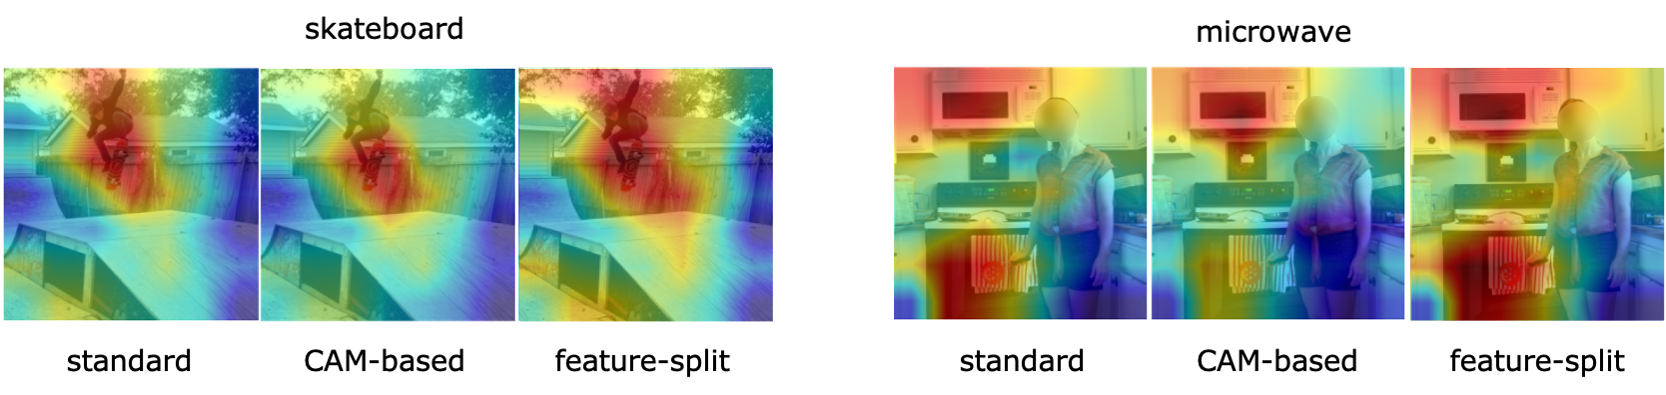
\includegraphics[width=0.99\linewidth]{../openreview/images/cams_skateboard_microwave.png}
    \caption{Biased category CAMs for (skateboard, person) and (microwave, oven) pairs.}
    \label{fig:cams}
\end{figure}


\section{Our additional experiments}

To better understand the proposed \emph{CAM-based} and \emph{feature-split} methods, we conducted several ablation studies (Table~\ref{tab:additionalexperiments}).\\
\\
\textbf{What is the effect of the regularization term in the \emph{CAM-based} method?} As mentioned in Section~\ref{sec:cam}, we tried varying the weight for the regularization term $L_R$ ($\lambda_2$) in the \emph{CAM-based} method that prevents the CAMs of the biased category pairs from drifting apart from the pixel regions of CAM$_{\text{pre}}$. We observed that weak regularization allows for highly localized, degenerate CAMs that don't resemble CAM$_{\text{pre}}$, while overly strong regularization makes the method less effective. We were able to strike an ideal balance with $\lambda_2$=0.1, higher than the paper's $\lambda_2$=0.01.\\
\\
\textbf{What is the effect of the weighted loss in the \emph{feature-split} method?} To understand the effect of the weighted loss in the \emph{feature-split} method, we tried training a \emph{feature-split} model without it and a baseline model with the \emph{feature-split} weighted loss. Both variations have lower ``exclusive" mAPs, suggesting that both the feature-splitting framework and the weighted loss are important components of the method. We highlight that the \emph{feature-split} model trained without the weighted loss is worse than the \emph{standard} model, suggesting that the weighted loss is central for the \emph{feature-split} method to achieve good performance. However, we also observed that the \emph{feature-split} method's weighted loss by itself is not sufficient for improving the performance of the \emph{standard} model on the ``exclusive" distribution.\\
\\
\textbf{Does the size of the \textit{feature-split} subspace matter?} In the \textit{feature-split} method, the original paper allocates half of the 2,048 feature dimensions in the fc layer for learning exclusive image examples. We explored whether a smaller or larger $\mathrm{x}_o$ subspace may strike a better balance and improve both ``exclusive" and ``co-occur" performance, as the number of exclusive images is only a small fraction of the entire training data. For COCO-Stuff, the performance peaks on ``exclusive" and dips on ``co-occur" at the 1,024 dimension split. For DeepFashion, performance on both distributions peak at the 1,024 dimension split. For AwA, however, the performance on both distributions improves as the subspace size increases. Lastly for UnRel, the model trained on COCO-stuff with a $\mathrm{x}_o$ of size 768 performs best. Overall, we did not find a clear trend between \emph{feature-split} performance and subspace size. 


\begin{table}[h!]
\centering
\caption{(Top) Ablation studies of \emph{CAM-based} and \emph{feature-split} on COCO-Stuff. (Bottom) Additional \emph{feature-split} results with varying $\mathrm{x}_o$ subspace sizes. Best results are in bold.}
\label{tab:additionalexperiments}
% \resizebox{0.72\linewidth}{!}{
\resizebox{0.99\linewidth}{!}{
\begin{tabular}{|l|c|c|c|c|}
\hline
Method & Exclusive & Co-occur & All & Non-biased \\
\hline
\textit{standard} & 23.9 & \textbf{65.0} & \textbf{55.7} & \textbf{72.3} \\
\hline
\textit{CAM-based} with $\lambda_2 = 0$ (no regularization) & 24.4 & 64.6 & 55.5 & 72.0 \\
\textit{CAM-based} with $\lambda_2 = 0.01$ (paper params) & 24.6 & 64.6 & 55.5 & 72.0 \\
\textit{CAM-based} with $\lambda_2 = 0.1$ (tuned params) & \textbf{26.9} & 64.2 & 55.5 & 72.2 \\
\hline
\textit{feature-split} & \textbf{28.1} & 64.8 & 55.6 & 72.1 \\
\textit{feature-split} without weighted loss & 23.6 & 65.4 & 55.6 & 72.1 \\
baseline with \textit{feature-split} weighted loss & 24.0 & 64.8 & 55.5 & 72.1 \\
\hline
\end{tabular}
}
\end{table}

\vspace{-0.3cm}

\begin{table}[h!]
\centering
% \resizebox{0.82\linewidth}{!}{
\resizebox{0.99\linewidth}{!}{
\begin{tabular}{|c|c|c|c|c|c|c|c|}
\hline
\multirow{2}{*}{$\mathrm{x}_o$ size} & \multicolumn{2}{c|}{COCO-Stuff (mAP)} & \multicolumn{2}{c|}{DeepFashion (top-3 recall)} & \multicolumn{2}{c|}{AwA (mAP)} & UnRel (mAP) \\
\cline{2-8}
& Exclusive & Co-occur & Exclusive & Co-occur & Exclusive & Co-occur & 3 categories \\
\cline{2-8}
\hline
256    & 23.8 & 65.9 & 3.2 & 12.5 & 18.5 & 69.7 & 47.8 \\
512    & 26.7 & 65.9 & 3.4 & 12.9 & 18.7 & 69.0 & 50.1 \\
768    & 27.2 & 65.8 & 4.6 & 14.3 & 19.1 & 69.2 & \textbf{50.4} \\
\hline
1,024  & \textbf{28.1} & 64.8 & \textbf{12.2} & \textbf{27.1} & 19.2 & 68.6 & 49.9 \\
\hline
1,280  & 24.8 & 66.0 & 4.0 & 13.7 & 19.3 & 69.9 & 45.8 \\
1,536  & 23.0 & 66.1 & 2.7 & 13.9 & 19.5 & 70.3 & 44.2 \\
1,792  & 21.7 & \textbf{66.2} & 2.3 & 14.1 & \textbf{19.7} & \textbf{70.8} & 40.6 \\
\hline
\end{tabular}
}
\end{table}

%\vspace{-0.3cm}